\documentclass[12pt]{exam}
\usepackage[utf8]{inputenc}

\usepackage[margin=1in]{geometry}
\usepackage{amsmath,amssymb}
\usepackage{multicol}
\usepackage{upquote}
\usepackage{url}
\newcommand{\class}{miniHive}
\newcommand{\term}{}
\newcommand{\examnum}{Milestone 4}
\newcommand{\examdate}{}
\usepackage{paralist}
\usepackage{fancyvrb}
\usepackage{graphicx}


\pagestyle{head}
\firstpageheader{}{}{}
\runningheader{\class}{\examnum\ - Page \thepage\ of \numpages}{}
\runningheadrule



\begin{document}

\noindent
\begin{tabular*}{\textwidth}{l @{\extracolsep{\fill}} r @{\extracolsep{6pt}} l}
\textbf{\class} & \\
\textbf{\term} &&\\
\textbf{\examnum} &&\\
\textbf{\examdate} &&\\
\end{tabular*}\\
\rule[2ex]{\textwidth}{2pt}

\noprintanswers

\noindent


\section*{Optimizing {\em miniHive}\/}

In the fourth milestone, we optimize {\em miniHive}\/.
 The goal is to reduce the total amount of data stored in intermediary files within HDFS.
 
We have considered various options in class, and it is up to you which optimization(s) you implement. Chain folding is a good bet. You may also implement more than one idea.

In case  you need to adapt the LUIGI workflow, there is a chapter from the book ``Hadoop with Python'' with an introduction to LUIGI in Moodle.


\section{Evaluation Data}

We use data from the TPC-H benchmark, describing customers and their orders. This is a famous benchmark, where synthetic data can be generated based on a scale factor (SF). 

The ER-like diagram in Figure~\ref{tpch} describes the schema, and has been taken from the official benchmark description. We assume that all  data adheres to this schema.

\begin{figure}[t]
\centering
    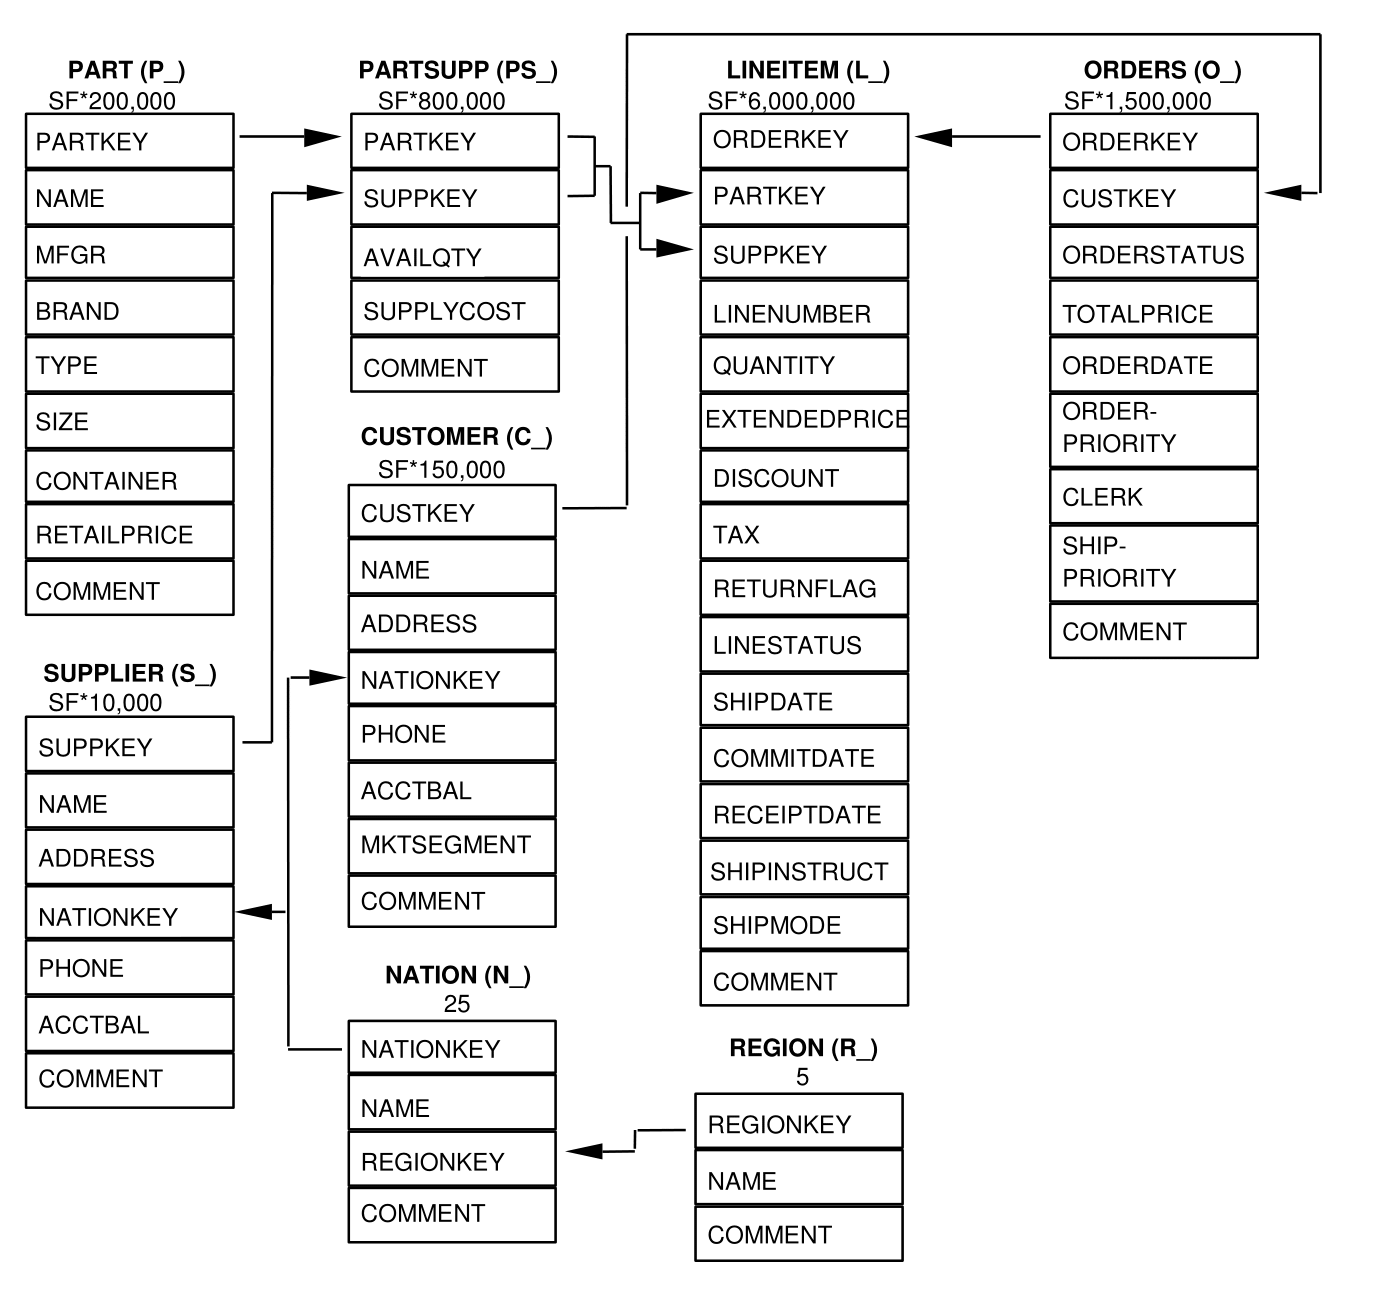
\includegraphics[scale=.3]{tpch.png}
    \caption{The TCP-H benchmark data [Source: {\tt www.tpc.org}.]}
    \label{tpch}
\end{figure}

The parentheses following each table name contain the prefix of the column names for that table.
The arrows point in the direction of the one-to-many relationships between tables.
The number/formula below each table name represents the cardinality (number of rows) of the table. Some are factored by SF, the scale factor. 


\section{Calling {\em miniHive}\/}



For evaluating a single query, {\em miniHive} gets 

\begin{compactitem}
    \item an optional flag telling miniHive to switch optimization on, 
    \item the optional scale factor, allowing you to derive the
 {\em approximate}\/ sizes of tables,
    \item the input files, already stored in HDFS or available as local files, 

    \item the optional execution environment (LOCAL or HDFS), set to HDFS by default,
        \item the SQL query over TPC-H data  to evaluate.
\end{compactitem}

\noindent
This is how we  call the optimized {\em miniHive}\/ for execution on local files:

\begin{Verbatim}[frame=single]
miniHive.py --O --SF 1 --env LOCAL "select distinct N_NAME from NATION"
\end{Verbatim}

If called in \verb!LOCAL! mode, this outputs an approximation of the HDFS storage costs (more on this later).
{\bf Make sure your submitted version does not write any other information to standard out, as this will confuse the test scripts.}

\section{Material in Moodle}

\begin{compactitem}

\item    
A sample dataset that was generated with scale factor~0.01 (\verb!data_0_01.zip!). 


\item 
The  file \verb!miniHive.py!. You may alter this file.

\item 
The file \verb!costcouter.py!. You must not alter this file.

\item
A list of SQL test queries in \verb!miniHive.q!.

\end{compactitem}



\section{What to Submit}

Submit a flat ZIP file (without any subfolders) containing

\begin{compactitem}
    \item a README file mentioning any additional Python modules that need to be installed via \verb!pip!, and a 1-paragraph description of the optimization(s) that you have implemented. The README must have this format:

    \begin{Verbatim}[frame=single,fontsize=\small]
# Author: <your lastname>, <your firstname>
# TODO install <comma-separated list of modules to install, or empty>
        
# My approach:
<1-paragraph description of your optimizations>
    \end{Verbatim}
    
    
    \item Further, all Python files required to run {\em miniHive}. 

\end{compactitem}







\end{document}